% Colin-N. Brosseau
% Juin 2016
%
% This document is based on 
% http://www.LaTeXTemplates.com
% Original author:
% Mathias Legrand (legrand.mathias@gmail.com) with modifications by:
% Vel (vel@latextemplates.com)
%
% License:
% CC BY-NC-SA 3.0 (http://creativecommons.org/licenses/by-nc-sa/3.0/)
%
% Compile it from the command line with the  commands below to make
% sure your LaTeX distribution is configured correctly:
%
%     pdflatex procedurierLeonelli
%     makeindex procedurierLeonelli.idx -s StyleInd.ist
%     pdflatex procedurierLeonelli 
%     pdflatex procedurierLeonelli 
%
% Easy compilation (latexmk needed)
%
%     make

%----------------------------------------------------------------------------------------
%	PACKAGES AND OTHER DOCUMENT CONFIGURATIONS
%----------------------------------------------------------------------------------------

%\documentclass[11pt,fleqn]{book} % Default font size and left-justified equations
\documentclass[11pt,francais]{book} % Default font size and left-justified equations

%\usepackage[francais]{babel}
\usepackage{babel}
\usepackage[utf8]{inputenc}
\usepackage[T1]{fontenc}

% Creative commons
\usepackage{cclicenses}

% Code source
\usepackage{listings}             % Include the listings-package

% Diagrammes (boites)
\usepackage{smartdiagram}

%----------------------------------------------------------------------------------------

%%%%%%%%%%%%%%%%%%%%%%%%%%%%%%%%%%%%%%%%%
% The Legrand Orange Book
% Structural Definitions File
% Version 2.0 (9/2/15)
%
% Original author:
% Mathias Legrand (legrand.mathias@gmail.com) with modifications by:
% Vel (vel@latextemplates.com)
% 
% This file has been downloaded from:
% http://www.LaTeXTemplates.com
%
% License:
% CC BY-NC-SA 3.0 (http://creativecommons.org/licenses/by-nc-sa/3.0/)
%
%%%%%%%%%%%%%%%%%%%%%%%%%%%%%%%%%%%%%%%%%

%----------------------------------------------------------------------------------------
%	VARIOUS REQUIRED PACKAGES AND CONFIGURATIONS
%----------------------------------------------------------------------------------------

\usepackage[top=3cm,bottom=3cm,left=3cm,right=3cm,headsep=10pt,a4paper]{geometry} % Page margins

\usepackage{graphicx} % Required for including pictures
\graphicspath{{Images/}} % Specifies the directory where pictures are stored

\usepackage{lipsum} % Inserts dummy text

\usepackage{tikz} % Required for drawing custom shapes

\usepackage[english]{babel} % English language/hyphenation

\usepackage{enumitem} % Customize lists
\setlist{nolistsep} % Reduce spacing between bullet points and numbered lists

\usepackage{booktabs} % Required for nicer horizontal rules in tables

\usepackage{xcolor} % Required for specifying colors by name
\definecolor{ocre}{RGB}{243,102,25} % Define the orange color used for highlighting throughout the book

%----------------------------------------------------------------------------------------
%	FONTS
%----------------------------------------------------------------------------------------

\usepackage{avant} % Use the Avantgarde font for headings
%\usepackage{times} % Use the Times font for headings
\usepackage{mathptmx} % Use the Adobe Times Roman as the default text font together with math symbols from the Sym­bol, Chancery and Com­puter Modern fonts

\usepackage{microtype} % Slightly tweak font spacing for aesthetics
\usepackage[utf8]{inputenc} % Required for including letters with accents
\usepackage[T1]{fontenc} % Use 8-bit encoding that has 256 glyphs

%----------------------------------------------------------------------------------------
%	BIBLIOGRAPHY AND INDEX
%----------------------------------------------------------------------------------------

\usepackage[style=alphabetic,citestyle=numeric,sorting=nyt,sortcites=true,autopunct=true,babel=hyphen,hyperref=true,abbreviate=false,backref=true,backend=biber]{biblatex}
\addbibresource{bibliography.bib} % BibTeX bibliography file
\defbibheading{bibempty}{}

\usepackage{calc} % For simpler calculation - used for spacing the index letter headings correctly
\usepackage{makeidx} % Required to make an index
\makeindex % Tells LaTeX to create the files required for indexing

%----------------------------------------------------------------------------------------
%	MAIN TABLE OF CONTENTS
%----------------------------------------------------------------------------------------

\usepackage{titletoc} % Required for manipulating the table of contents

\contentsmargin{0cm} % Removes the default margin

% Part text styling
\titlecontents{part}[0cm]
{\addvspace{20pt}\centering\large\bfseries}
{}
{}
{}

% Chapter text styling
\titlecontents{chapter}[1.25cm] % Indentation
{\addvspace{12pt}\large\sffamily\bfseries} % Spacing and font options for chapters
{\color{ocre!60}\contentslabel[\Large\thecontentslabel]{1.25cm}\color{ocre}} % Chapter number
{\color{ocre}}  
{\color{ocre!60}\normalsize\;\titlerule*[.5pc]{.}\;\thecontentspage} % Page number

% Section text styling
\titlecontents{section}[1.25cm] % Indentation
{\addvspace{3pt}\sffamily\bfseries} % Spacing and font options for sections
{\contentslabel[\thecontentslabel]{1.25cm}} % Section number
{}
{\hfill\color{black}\thecontentspage} % Page number
[]

% Subsection text styling
\titlecontents{subsection}[1.25cm] % Indentation
{\addvspace{1pt}\sffamily\small} % Spacing and font options for subsections
{\contentslabel[\thecontentslabel]{1.25cm}} % Subsection number
{}
{\ \titlerule*[.5pc]{.}\;\thecontentspage} % Page number
[]

% List of figures
\titlecontents{figure}[0em]
{\addvspace{-5pt}\sffamily}
{\thecontentslabel\hspace*{1em}}
{}
{\ \titlerule*[.5pc]{.}\;\thecontentspage}
[]

% List of tables
\titlecontents{table}[0em]
{\addvspace{-5pt}\sffamily}
{\thecontentslabel\hspace*{1em}}
{}
{\ \titlerule*[.5pc]{.}\;\thecontentspage}
[]

%----------------------------------------------------------------------------------------
%	MINI TABLE OF CONTENTS IN PART HEADS
%----------------------------------------------------------------------------------------

% Chapter text styling
\titlecontents{lchapter}[0em] % Indenting
{\addvspace{15pt}\large\sffamily\bfseries} % Spacing and font options for chapters
{\color{ocre}\contentslabel[\Large\thecontentslabel]{1.25cm}\color{ocre}} % Chapter number
{}  
{\color{ocre}\normalsize\sffamily\bfseries\;\titlerule*[.5pc]{.}\;\thecontentspage} % Page number

% Section text styling
\titlecontents{lsection}[0em] % Indenting
{\sffamily\small} % Spacing and font options for sections
{\contentslabel[\thecontentslabel]{1.25cm}} % Section number
{}
{}

% Subsection text styling
\titlecontents{lsubsection}[.5em] % Indentation
{\normalfont\footnotesize\sffamily} % Font settings
{}
{}
{}

%----------------------------------------------------------------------------------------
%	PAGE HEADERS
%----------------------------------------------------------------------------------------

\usepackage{fancyhdr} % Required for header and footer configuration

\pagestyle{fancy}
\renewcommand{\chaptermark}[1]{\markboth{\sffamily\normalsize\bfseries\chaptername\ \thechapter.\ #1}{}} % Chapter text font settings
\renewcommand{\sectionmark}[1]{\markright{\sffamily\normalsize\thesection\hspace{5pt}#1}{}} % Section text font settings
\fancyhf{} \fancyhead[LE,RO]{\sffamily\normalsize\thepage} % Font setting for the page number in the header
\fancyhead[LO]{\rightmark} % Print the nearest section name on the left side of odd pages
\fancyhead[RE]{\leftmark} % Print the current chapter name on the right side of even pages
\renewcommand{\headrulewidth}{0.5pt} % Width of the rule under the header
\addtolength{\headheight}{2.5pt} % Increase the spacing around the header slightly
\renewcommand{\footrulewidth}{0pt} % Removes the rule in the footer
\fancypagestyle{plain}{\fancyhead{}\renewcommand{\headrulewidth}{0pt}} % Style for when a plain pagestyle is specified

% Removes the header from odd empty pages at the end of chapters
\makeatletter
\renewcommand{\cleardoublepage}{
\clearpage\ifodd\c@page\else
\hbox{}
\vspace*{\fill}
\thispagestyle{empty}
\newpage
\fi}

%----------------------------------------------------------------------------------------
%	THEOREM STYLES
%----------------------------------------------------------------------------------------

\usepackage{amsmath,amsfonts,amssymb,amsthm} % For math equations, theorems, symbols, etc

\newcommand{\intoo}[2]{\mathopen{]}#1\,;#2\mathclose{[}}
\newcommand{\ud}{\mathop{\mathrm{{}d}}\mathopen{}}
\newcommand{\intff}[2]{\mathopen{[}#1\,;#2\mathclose{]}}
\newtheorem{notation}{Notation}[chapter]

% Boxed/framed environments
\newtheoremstyle{ocrenumbox}% % Theorem style name
{0pt}% Space above
{0pt}% Space below
{\normalfont}% % Body font
{}% Indent amount
{\small\bf\sffamily\color{ocre}}% % Theorem head font
{\;}% Punctuation after theorem head
{0.25em}% Space after theorem head
{\small\sffamily\color{ocre}\thmname{#1}\nobreakspace\thmnumber{\@ifnotempty{#1}{}\@upn{#2}}% Theorem text (e.g. Theorem 2.1)
\thmnote{\nobreakspace\the\thm@notefont\sffamily\bfseries\color{black}---\nobreakspace#3.}} % Optional theorem note
\renewcommand{\qedsymbol}{$\blacksquare$}% Optional qed square

\newtheoremstyle{blacknumex}% Theorem style name
{5pt}% Space above
{5pt}% Space below
{\normalfont}% Body font
{} % Indent amount
{\small\bf\sffamily}% Theorem head font
{\;}% Punctuation after theorem head
{0.25em}% Space after theorem head
{\small\sffamily{\tiny\ensuremath{\blacksquare}}\nobreakspace\thmname{#1}\nobreakspace\thmnumber{\@ifnotempty{#1}{}\@upn{#2}}% Theorem text (e.g. Theorem 2.1)
\thmnote{\nobreakspace\the\thm@notefont\sffamily\bfseries---\nobreakspace#3.}}% Optional theorem note

\newtheoremstyle{blacknumbox} % Theorem style name
{0pt}% Space above
{0pt}% Space below
{\normalfont}% Body font
{}% Indent amount
{\small\bf\sffamily}% Theorem head font
{\;}% Punctuation after theorem head
{0.25em}% Space after theorem head
{\small\sffamily\thmname{#1}\nobreakspace\thmnumber{\@ifnotempty{#1}{}\@upn{#2}}% Theorem text (e.g. Theorem 2.1)
\thmnote{\nobreakspace\the\thm@notefont\sffamily\bfseries---\nobreakspace#3.}}% Optional theorem note

% Non-boxed/non-framed environments
\newtheoremstyle{ocrenum}% % Theorem style name
{5pt}% Space above
{5pt}% Space below
{\normalfont}% % Body font
{}% Indent amount
{\small\bf\sffamily\color{ocre}}% % Theorem head font
{\;}% Punctuation after theorem head
{0.25em}% Space after theorem head
{\small\sffamily\color{ocre}\thmname{#1}\nobreakspace\thmnumber{\@ifnotempty{#1}{}\@upn{#2}}% Theorem text (e.g. Theorem 2.1)
\thmnote{\nobreakspace\the\thm@notefont\sffamily\bfseries\color{black}---\nobreakspace#3.}} % Optional theorem note
\renewcommand{\qedsymbol}{$\blacksquare$}% Optional qed square
\makeatother

% Defines the theorem text style for each type of theorem to one of the three styles above
\newcounter{dummy} 
\numberwithin{dummy}{section}
\theoremstyle{ocrenumbox}
\newtheorem{theoremeT}[dummy]{Theorem}
\newtheorem{problem}{Problem}[chapter]
\newtheorem{exerciseT}{Exercise}[chapter]
\theoremstyle{blacknumex}
\newtheorem{exampleT}{Example}[chapter]
\theoremstyle{blacknumbox}
\newtheorem{vocabulary}{Vocabulary}[chapter]
\newtheorem{definitionT}{Definition}[section]
\newtheorem{corollaryT}[dummy]{Corollary}
\theoremstyle{ocrenum}
\newtheorem{proposition}[dummy]{Proposition}

%----------------------------------------------------------------------------------------
%	DEFINITION OF COLORED BOXES
%----------------------------------------------------------------------------------------

\RequirePackage[framemethod=default]{mdframed} % Required for creating the theorem, definition, exercise and corollary boxes

% Theorem box
\newmdenv[skipabove=7pt,
skipbelow=7pt,
backgroundcolor=black!5,
linecolor=ocre,
innerleftmargin=5pt,
innerrightmargin=5pt,
innertopmargin=5pt,
leftmargin=0cm,
rightmargin=0cm,
innerbottommargin=5pt]{tBox}

% Exercise box	  
\newmdenv[skipabove=7pt,
skipbelow=7pt,
rightline=false,
leftline=true,
topline=false,
bottomline=false,
backgroundcolor=ocre!10,
linecolor=ocre,
innerleftmargin=5pt,
innerrightmargin=5pt,
innertopmargin=5pt,
innerbottommargin=5pt,
leftmargin=0cm,
rightmargin=0cm,
linewidth=4pt]{eBox}	

% Definition box
\newmdenv[skipabove=7pt,
skipbelow=7pt,
rightline=false,
leftline=true,
topline=false,
bottomline=false,
linecolor=ocre,
innerleftmargin=5pt,
innerrightmargin=5pt,
innertopmargin=0pt,
leftmargin=0cm,
rightmargin=0cm,
linewidth=4pt,
innerbottommargin=0pt]{dBox}	

% Corollary box
\newmdenv[skipabove=7pt,
skipbelow=7pt,
rightline=false,
leftline=true,
topline=false,
bottomline=false,
linecolor=gray,
backgroundcolor=black!5,
innerleftmargin=5pt,
innerrightmargin=5pt,
innertopmargin=5pt,
leftmargin=0cm,
rightmargin=0cm,
linewidth=4pt,
innerbottommargin=5pt]{cBox}

% Creates an environment for each type of theorem and assigns it a theorem text style from the "Theorem Styles" section above and a colored box from above
\newenvironment{theorem}{\begin{tBox}\begin{theoremeT}}{\end{theoremeT}\end{tBox}}
\newenvironment{exercise}{\begin{eBox}\begin{exerciseT}}{\hfill{\color{ocre}\tiny\ensuremath{\blacksquare}}\end{exerciseT}\end{eBox}}				  
\newenvironment{definition}{\begin{dBox}\begin{definitionT}}{\end{definitionT}\end{dBox}}	
\newenvironment{example}{\begin{exampleT}}{\hfill{\tiny\ensuremath{\blacksquare}}\end{exampleT}}		
\newenvironment{corollary}{\begin{cBox}\begin{corollaryT}}{\end{corollaryT}\end{cBox}}	

%----------------------------------------------------------------------------------------
%	REMARK ENVIRONMENT
%----------------------------------------------------------------------------------------

\newenvironment{remark}{\par\vspace{10pt}\small % Vertical white space above the remark and smaller font size
\begin{list}{}{
\leftmargin=35pt % Indentation on the left
\rightmargin=25pt}\item\ignorespaces % Indentation on the right
\makebox[-2.5pt]{\begin{tikzpicture}[overlay]
\node[draw=ocre!60,line width=1pt,circle,fill=ocre!25,font=\sffamily\bfseries,inner sep=2pt,outer sep=0pt] at (-15pt,0pt){\textcolor{ocre}{R}};\end{tikzpicture}} % Orange R in a circle
\advance\baselineskip -1pt}{\end{list}\vskip5pt} % Tighter line spacing and white space after remark

%----------------------------------------------------------------------------------------
%	SECTION NUMBERING IN THE MARGIN
%----------------------------------------------------------------------------------------

\makeatletter
\renewcommand{\@seccntformat}[1]{\llap{\textcolor{ocre}{\csname the#1\endcsname}\hspace{1em}}}                    
\renewcommand{\section}{\@startsection{section}{1}{\z@}
{-4ex \@plus -1ex \@minus -.4ex}
{1ex \@plus.2ex }
{\normalfont\large\sffamily\bfseries}}
\renewcommand{\subsection}{\@startsection {subsection}{2}{\z@}
{-3ex \@plus -0.1ex \@minus -.4ex}
{0.5ex \@plus.2ex }
{\normalfont\sffamily\bfseries}}
\renewcommand{\subsubsection}{\@startsection {subsubsection}{3}{\z@}
{-2ex \@plus -0.1ex \@minus -.2ex}
{.2ex \@plus.2ex }
{\normalfont\small\sffamily\bfseries}}                        
\renewcommand\paragraph{\@startsection{paragraph}{4}{\z@}
{-2ex \@plus-.2ex \@minus .2ex}
{.1ex}
{\normalfont\small\sffamily\bfseries}}

%----------------------------------------------------------------------------------------
%	PART HEADINGS
%----------------------------------------------------------------------------------------

% numbered part in the table of contents
\newcommand{\@mypartnumtocformat}[2]{%
\setlength\fboxsep{0pt}%
\noindent\colorbox{ocre!20}{\strut\parbox[c][.7cm]{\ecart}{\color{ocre!70}\Large\sffamily\bfseries\centering#1}}\hskip\esp\colorbox{ocre!40}{\strut\parbox[c][.7cm]{\linewidth-\ecart-\esp}{\Large\sffamily\centering#2}}}%
%%%%%%%%%%%%%%%%%%%%%%%%%%%%%%%%%%
% unnumbered part in the table of contents
\newcommand{\@myparttocformat}[1]{%
\setlength\fboxsep{0pt}%
\noindent\colorbox{ocre!40}{\strut\parbox[c][.7cm]{\linewidth}{\Large\sffamily\centering#1}}}%
%%%%%%%%%%%%%%%%%%%%%%%%%%%%%%%%%%
\newlength\esp
\setlength\esp{4pt}
\newlength\ecart
\setlength\ecart{1.2cm-\esp}
\newcommand{\thepartimage}{}%
\newcommand{\partimage}[1]{\renewcommand{\thepartimage}{#1}}%
\def\@part[#1]#2{%
\ifnum \c@secnumdepth >-2\relax%
\refstepcounter{part}%
\addcontentsline{toc}{part}{\texorpdfstring{\protect\@mypartnumtocformat{\thepart}{#1}}{\partname~\thepart\ ---\ #1}}
\else%
\addcontentsline{toc}{part}{\texorpdfstring{\protect\@myparttocformat{#1}}{#1}}%
\fi%
\startcontents%
\markboth{}{}%
{\thispagestyle{empty}%
\begin{tikzpicture}[remember picture,overlay]%
\node at (current page.north west){\begin{tikzpicture}[remember picture,overlay]%	
\fill[ocre!20](0cm,0cm) rectangle (\paperwidth,-\paperheight);
\node[anchor=north] at (4cm,-3.25cm){\color{ocre!40}\fontsize{220}{100}\sffamily\bfseries\@Roman\c@part}; 
\node[anchor=south east] at (\paperwidth-1cm,-\paperheight+1cm){\parbox[t][][t]{8.5cm}{
\printcontents{l}{0}{\setcounter{tocdepth}{1}}%
}};
\node[anchor=north east] at (\paperwidth-1.5cm,-3.25cm){\parbox[t][][t]{15cm}{\strut\raggedleft\color{white}\fontsize{30}{30}\sffamily\bfseries#2}};
\end{tikzpicture}};
\end{tikzpicture}}%
\@endpart}
\def\@spart#1{%
\startcontents%
\phantomsection
{\thispagestyle{empty}%
\begin{tikzpicture}[remember picture,overlay]%
\node at (current page.north west){\begin{tikzpicture}[remember picture,overlay]%	
\fill[ocre!20](0cm,0cm) rectangle (\paperwidth,-\paperheight);
\node[anchor=north east] at (\paperwidth-1.5cm,-3.25cm){\parbox[t][][t]{15cm}{\strut\raggedleft\color{white}\fontsize{30}{30}\sffamily\bfseries#1}};
\end{tikzpicture}};
\end{tikzpicture}}
\addcontentsline{toc}{part}{\texorpdfstring{%
\setlength\fboxsep{0pt}%
\noindent\protect\colorbox{ocre!40}{\strut\protect\parbox[c][.7cm]{\linewidth}{\Large\sffamily\protect\centering #1\quad\mbox{}}}}{#1}}%
\@endpart}
\def\@endpart{\vfil\newpage
\if@twoside
\if@openright
\null
\thispagestyle{empty}%
\newpage
\fi
\fi
\if@tempswa
\twocolumn
\fi}

%----------------------------------------------------------------------------------------
%	CHAPTER HEADINGS
%----------------------------------------------------------------------------------------

% A switch to conditionally include a picture, implemented by  Christian Hupfer
\newif\ifusechapterimage
\usechapterimagetrue
\newcommand{\thechapterimage}{}%
\newcommand{\chapterimage}[1]{\ifusechapterimage\renewcommand{\thechapterimage}{#1}\fi}%
\def\@makechapterhead#1{%
{\parindent \z@ \raggedright \normalfont
\ifnum \c@secnumdepth >\m@ne
\if@mainmatter
\begin{tikzpicture}[remember picture,overlay]
\node at (current page.north west)
{\begin{tikzpicture}[remember picture,overlay]
\node[anchor=north west,inner sep=0pt] at (0,0) {\ifusechapterimage\includegraphics[width=\paperwidth]{\thechapterimage}\fi};
\draw[anchor=west] (\Gm@lmargin,-9cm) node [line width=2pt,rounded corners=15pt,draw=ocre,fill=white,fill opacity=0.5,inner sep=15pt]{\strut\makebox[22cm]{}};
\draw[anchor=west] (\Gm@lmargin+.3cm,-9cm) node {\huge\sffamily\bfseries\color{black}\thechapter. #1\strut};
\end{tikzpicture}};
\end{tikzpicture}
\else
\begin{tikzpicture}[remember picture,overlay]
\node at (current page.north west)
{\begin{tikzpicture}[remember picture,overlay]
\node[anchor=north west,inner sep=0pt] at (0,0) {\ifusechapterimage\includegraphics[width=\paperwidth]{\thechapterimage}\fi};
\draw[anchor=west] (\Gm@lmargin,-9cm) node [line width=2pt,rounded corners=15pt,draw=ocre,fill=white,fill opacity=0.5,inner sep=15pt]{\strut\makebox[22cm]{}};
\draw[anchor=west] (\Gm@lmargin+.3cm,-9cm) node {\huge\sffamily\bfseries\color{black}#1\strut};
\end{tikzpicture}};
\end{tikzpicture}
\fi\fi\par\vspace*{270\p@}}}

%-------------------------------------------

\def\@makeschapterhead#1{%
\begin{tikzpicture}[remember picture,overlay]
\node at (current page.north west)
{\begin{tikzpicture}[remember picture,overlay]
\node[anchor=north west,inner sep=0pt] at (0,0) {\ifusechapterimage\includegraphics[width=\paperwidth]{\thechapterimage}\fi};
\draw[anchor=west] (\Gm@lmargin,-9cm) node [line width=2pt,rounded corners=15pt,draw=ocre,fill=white,fill opacity=0.5,inner sep=15pt]{\strut\makebox[22cm]{}};
\draw[anchor=west] (\Gm@lmargin+.3cm,-9cm) node {\huge\sffamily\bfseries\color{black}#1\strut};
\end{tikzpicture}};
\end{tikzpicture}
\par\vspace*{270\p@}}
\makeatother

%----------------------------------------------------------------------------------------
%	HYPERLINKS IN THE DOCUMENTS
%----------------------------------------------------------------------------------------

\usepackage{hyperref}
\hypersetup{hidelinks,backref=true,pagebackref=true,hyperindex=true,colorlinks=false,breaklinks=true,urlcolor= ocre,bookmarks=true,bookmarksopen=false,pdftitle={Title},pdfauthor={Author}}
\usepackage{bookmark}
\bookmarksetup{
open,
numbered,
addtohook={%
\ifnum\bookmarkget{level}=0 % chapter
\bookmarksetup{bold}%
\fi
\ifnum\bookmarkget{level}=-1 % part
\bookmarksetup{color=ocre,bold}%
\fi
}
}
 % Insert the commands.tex file which contains the majority of the structure behind the template

\begin{document}

\renewcommand{\lstlistingname}{Code}

%----------------------------------------------------------------------------------------
%	TITLE PAGE
%----------------------------------------------------------------------------------------

\begingroup
\thispagestyle{empty}
\begin{tikzpicture}[remember picture,overlay]
\coordinate [below=12cm] (midpoint) at (current page.north);
\node at (current page.north west)
{\begin{tikzpicture}[remember picture,overlay]
%\node[anchor=north west,inner sep=0pt] at (0,0) {
\includegraphics[width=\paperwidth,bb=0 0 100 100]{background}}; % Background image
\node[anchor=north west,inner sep=0pt] at (0,0) {
\includegraphics[width=\paperwidth]{background}}; % Background image
\draw[anchor=north] (midpoint) node [fill=ocre!30!white,fill opacity=0.6,text opacity=1,inner sep=1cm]{\Huge\centering\bfseries\sffamily\parbox[c][][t]{\paperwidth}{\centering Procédurier\\[15pt] % Book title
{\Large Laboratoire R. Leonelli}\\[20pt] % Subtitle
{\Large Colin-N. Brosseau}}}; % Author name
\end{tikzpicture}};
\end{tikzpicture}
\vfill
\endgroup

%----------------------------------------------------------------------------------------
%	COPYRIGHT PAGE
%----------------------------------------------------------------------------------------

\newpage
~\vfill
\thispagestyle{empty}

%\doclicenseThis

\noindent Copyright \copyright\ 2016 Colin-N. Brosseau\\ % Copyright notice

%\noindent \textsc{Published by Publisher}\\ % Publisher

\noindent \textsc{https://github.com/ColinBrosseau/LaboratoireLeonelli}\\ % URL

\noindent \cc \ccnc \bysa

\noindent Texte licensé sous licence Creative Commons attribution, pas d’utilisation commerciale, partage dans les mêmes conditions \url{http://creativecommons.org/licenses/by-nc-sa/3.0/fr/}.

%\noindent \textit{Première édition, Juillet 2016} % Printing/edition date
\noindent \textit{Édition 0.1, Juin 2016} % Printing/edition date

%----------------------------------------------------------------------------------------
%	TABLE OF CONTENTS
%----------------------------------------------------------------------------------------

%\usechapterimagefalse % If you don't want to include a chapter image, use this to toggle images off - it can be enabled later with \usechapterimagetrue

\chapterimage{laser} % Table of contents heading image

%\usechapterimagefalse % If you don't want to include a chapter image, use this to toggle images off - it can be enabled later with \usechapterimagetrue

\pagestyle{empty} % No headers

\tableofcontents % Print the table of contents itself

\cleardoublepage % Forces the first chapter to start on an odd page so it's on the right

\pagestyle{fancy} % Print headers again

%----------------------------------------------------------------------------------------
%	PART
%----------------------------------------------------------------------------------------

\part{Première partie}
 
%----------------------------------------------------------------------------------------
%	CHAPTER 1
%----------------------------------------------------------------------------------------

\chapterimage{laser} % Chapter heading image

\chapter{Logiciels}

De nombreux logiciels ont été mis au point dans le but de contrôler les nombreux appareils et expériences du laboratoire.
En général, les expériences et appareils fonctionnant dans le laboratoire {\it Trivista} utilisent Matlab.
De son côté, le laboratoire {\it U1000} est complètement implémenté avec Python\footnote{De nombreux appareils du laboratoire {\it U1000}~ont un interface Matlab, mais aucune mise à jour n'est faite depuis un moment.}.

\section{Matlab}%\index{Matlab}

À moins d'indication contraire, les codes Matlab utilisés au laboratoire ont été testés avec la version 7.1 (R14).

\subsection{Codes supplémentaires}

Plusieurs instruments sont contrôlés par cable GPIB.
On utilise deux ``modules'' associés:
\begin{itemize}
\item http://www.mathworks.com/matlabcentral/fileexchange/216
\item http://www.mathworks.com/matlabcentral/fileexchange/3140
%\caption{Modules GPIB utilisés par Matlab}
\label{tableModulesGPIBMatlab}
\end{itemize}
Les deux sont complémentaires.
Le premier, de Tom Davis, sert à la communication.
Le deuxième, d'Alaa Makdissi, est surtout utilisé pour l'initialisation.

\section{Python}\index{Python}

Plusieurs instruments du laboratoire peuvent être contrôlés avec Python.
En général, il s'agit des instruments situés dans le D405 (Labo Raman).

À l'heure actuelle, la manière la plus simple d'installer python sur windows est d'utiliser la {\bf distribution anaconda} https://www.continuum.io/downloads.
Il existe deux branches de Python soient la 2 et la 3. On prend {\bf Python 3}.

\subsection{Modules}

L'installation de base d'anaconda contient la plupart des modules nécessaires au fonctionnement des scripts utilisés dans le laboratoire.
On installe des des modules supplémentaires de la facon suivante (??? à compléter):
\begin{itemize}
\item ligne de commande
\item pip
\end{itemize}

Les modules nécessaires pour pouvoir utiliser les scripts concu pour le laboratoire sont énumérés dans la table \ref{tableModulesNecessaires}.

\begin{table}[]
\centering
\resizebox{\textwidth}{!}{%
\begin{tabular}{ll}
\multicolumn{1}{c}{\textbf{Module}} & \multicolumn{1}{c}{\textbf{Rôle}}                                \\ \hline
visa                                & contrôle des instruments (RS232, GPIB)                           \\
struct                              & utilisé par SR830c pour lire le flux binaire                     \\
yaml                                & lire/écrire des fichiers sous format YAML                        \\
collections                         & utilisé pour créer des dictionnaires ordonnés                    \\
pandas                              & manipulation simplifiée des structures des données scientifiques \\
matplotlib                          & tracer des graphiques                                            \\
\end{tabular}%
}
\caption{Modules nécessaires au fonctionnement des scripts du laboratoire}
\label{tableModulesNecessaires}
\end{table}

\subsubsection{visa}\index{visa}

Le module {\it visa}\footnote{\url{https://pyvisa.readthedocs.io/en/stable/}} permet d'interagir facilement avec les instruments du laboratoire.
Il nécessite que {\it LabView} soit installé sur l'ordinateur (??? confirmer).
Le Code~\ref{lst:exVisa} montre un exemple minimal de son utilisation.

\begin{lstlisting}[frame=single,caption={Exemple d'utilisation de {\it visa}},label={lst:exVisa},breaklines=true,]  % Start your code-block
 
import visa  # importe le module
rm = visa.ResourceManager()

# affiche la liste des appareils connectes
rm.list_resources()  
# ex. de sortie:
#     ('ASRL1::INSTR', 'ASRL2::INSTR', 'GPIB0::12::INSTR')

# initialise la communication
inst = rm.open_resource('GPIB0::12::INSTR')  # appareil connecte sur le permier interface GPIB a l'adresse 12

# questionne l'appareil
print(inst.query("*IDN?"))  # indenfication de l'appareil (commande typique)

# Ce qui suit est equivalent a query, mais en deux etapes

# ecrit dans l'appareil
inst.write("*IDN?")

# lit la reponse de l'appareil
print(inst.read("*IDN?"))

\end{lstlisting}

\subsubsection{Matplotlib}

\subsubsection{Pandas}



%----------------------------------------------------------------------------------------
%	CHAPTER 2
%----------------------------------------------------------------------------------------

\chapter{Instruments}

%----------------------------------------------------------------------------------------

\section{Bomem}\index{Bomem}

\subsection{Détecteur Silicium}

\subsection{Détecteur InGaAs}

Le détecteur InGaAs\footnote{Numéro de modèle: J23D-M205-R01M-60-1.9, http://www.teledynejudson.com/files/pdf/ingaas\_PB4206.pdf} est sensible dans la gamme 1000 - 1900 nm\footnote{La longueur d'onde maximale détectée dépend de la température. Elle est de 1900 nm à 20 $^{\circ}$C) mais passe à 1810 nm à -85 $^{\circ}$C. Une estimation rapide porte la longueur d'onde maximale à $\approx$ 1750 nm à température de l'azote liquide.}.

Ce détecteur a besoin d'azote liquide pour fonctionner.
Il est recommandé de pomper le vide d'isolation tous les 6 mois.

Le signal de ce détecteur est amplifié\footnote{Amplificateur PA-7-70, RD=70 G$\Omega$, CD=870 pF, RS=10.36 $\Omega$}.
Pour l'utilisation avec le Bomem, on utilise la sortie DC (premier étage).

\begin{figure}[h]
  \centering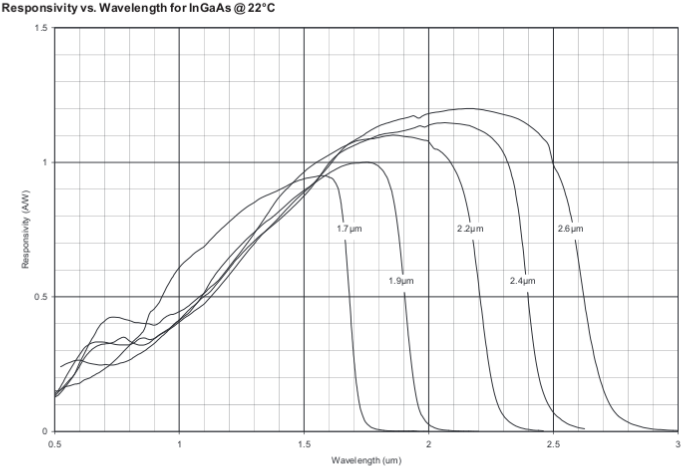
\includegraphics[width=.5\linewidth,height=7cm,keepaspectratio]{Bomem-InGaAs-Sensibilite-LongueurOnde}
  \caption{Sensibilité détecteur Bomem InGaAs (à 20 $^{\circ}$C)}
  \label{fig:pdaingaas}
\end{figure}



\subsection{Détecteur InSb}
Le détecteur InSb\footnote{Numéro de modèle: J10D-M204-R01M-60-SP28, http://www.judsontechnologies.com/files/pdf/InSb\_shortform\_Mar2003.pdf} est sensible dans la gamme 1000-2800 nm.

Ce détecteur a besoin d'azote liquide pour fonctionner.
Il est recommandé de pomper le vide d'isolation tous les 6 mois.

Le signal de ce détecteur est amplifié\footnote{Amplificateur PA-9, RD=150 M$\Omega$, CD=355 pF}.
Pour l'utilisation avec le Bomem, on utilise la sortie DC (premier étage).

\begin{figure}[h]
  \centering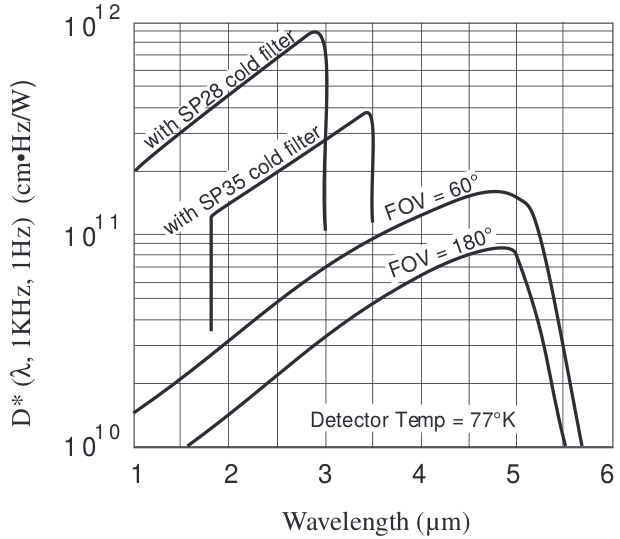
\includegraphics[width=.5\linewidth,height=7cm,keepaspectratio]{Bomem-InSb-Sensibilite-LongueurOnde}
  \caption{Sensibilité détecteur Bomem InSb (à 77 K)}
  \label{fig:pdaingaas}
\end{figure}


%----------------------------------------------------------------------------------------

\section{Caméras Princeton Instruments}

Les caméras Princeton Instruments (la PDA InGaAs et la Pixis) sont contrôlées soit par le logiciel Winspec ou par Matlab.
Les deux sont mutuellement exclusifs à un instant donné.

Lorsqu'on change de détecteur (passant de la PDA à la Pixis ou inversement), il {\bf faut} redémarrer Winspec et faire la procédure de détection.
Parfois ca ne fonctionne pas et il faut débrancher le cable USB du Trivista.

\subsection{Winspec}

Winspec permet de vérifier que la caméra fonctionne et tester rapidement le signal.
Il n'y a pas de calibration Pixel $\rightarrow$ Longueur d'onde.

\subsection{Matlab}

Matlab peut contrôler les caméras Princeton Instruments via la librairie pvcam:
\begin{center}
  \smartdiagramset{border color=none,
    uniform color list=gray!100!black for 10 items,
    back arrow disabled=true,}
  \smartdiagram[flow diagram:horizontal]{Matlab, pvcam, Caméra Princeton Instruments}
\end{center}

%\smartdiagram[flow diagram:horizontal,back arrow disabled=false,]{Matlab,  pvcam, Caméra Princeton Instruments}

\begin{lstlisting}[frame=single,caption={Exemple d'utilisation des caméras Princeton Instruments avec Matlab},label={lst:excameraprincetoninstruments},breaklines=true,]  % Start your code-block

???
\end{lstlisting}

\subsection{PDA InGaAs}\index{PDA InGaAs}

Ce détecteur est une rangée de 1024 pixels sensibles jusqu'à 2.2 $\mu$m (à température pièce ???).

Ce détecteur a besoin d'azote liquide pour fonctionner et on stabilise la température à -100 $^{\circ}$C.
Il {\bf doit} être connecté à son contrôleur (allumé) lorsqu'il y a de l'azote dans le réservoir.

Il est recommandé de pomper le vide d'isolation tous les 6 mois.

Étant donné qu'il est sensible à l'infrarouge, le bruit thermique est particulièrement important sur ce détecteur.
En général, on mesure 30 000 comptes {\it noirs} par seconde.
Étant donné que ce détecteur sature à 64 000 comptes, on limite l'accumulation à une seconde.

On peut contrôler ce détecteur avec la fonction Matlab générique ???.

\begin{figure}[h]
  \centering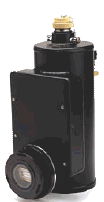
\includegraphics[width=.5\linewidth,height=7cm,keepaspectratio]{pdaInGaAs}
  \caption{PDA InGaAs}
  \label{fig:pdaingaas}
\end{figure}

\subsection{Pixis}\index{Pixis}

La caméra Pixis (Pixis 256) est composé de 1024x256 pixels sensibles jusqu'à $\approx$ 1 $\mu$m.
Elle est refroidie par effet Pelletier à -70 $^{\circ}$C.

Cette caméra a un bruit de lecture d'environ 600 comptes et un bruit noir suffisamment bas pour être négligeable dans la plupart des cas.

Tout comme la PDA InGaAS, on peut contrôler ce détecteur avec la fonction Matlab générique ???.

\begin{figure}[h]
  \centering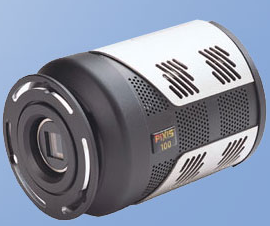
\includegraphics[width=.5\linewidth]{pixis}
  \caption{Pixis}
  \label{fig:pixis}
\end{figure}


%----------------------------------------------------------------------------------------

\section{CCD Raman}\index{CCD Raman}
%\section{Winspec}\index{Winspec}

La caméra CCD fixée sur le U1000 est composé de 1340x400 pixels sensibles jusqu'à $\approx$ 1 $\mu$m.

Cette caméra est refroidie par effet Pelletier à -100 $^{\circ}$C.
Elle {\bf doit} être connectée à son contrôleur (allumé) lorsqu'il y a de l'azote dans le réservoir.

Il est recommandé de pomper le vide d'isolation tous les 6 mois.

Ce détecteur a besoin de Winspec\footnote{ou Winview ???} pour pouvoir être contrôlée.
En plus de l'acquisition manuelle par Winspec, il est possible de le faire avec Python.
Cette dernière option permet d'automatiser l'acquisition.

\subsection{Python}

Le contrôle de la caméra par Python fonctionne selon le schéma suivant: 
\begin{center}
  \smartdiagramset{border color=none,
    uniform color list=gray!100!black for 10 items,
    back arrow disabled=true,}
  \smartdiagram[flow diagram:horizontal]{Python, Winspec, CCD Raman}
\end{center}

Il est donc nécessaire que Winspec soit en fonction lors de cette opération.
Un exemple minimal est donné dans Code~\ref{lst:exwinspec}.

\begin{lstlisting}[frame=single,caption={Exemple d'utilisation de Winspec avec Python},label={lst:exwinspec},breaklines=true,]  % Start your code-block

???
\end{lstlisting}

%----------------------------------------------------------------------------------------

\section{HydraHarp}\index{HydraHarp}

\begin{figure}[h]
  \centering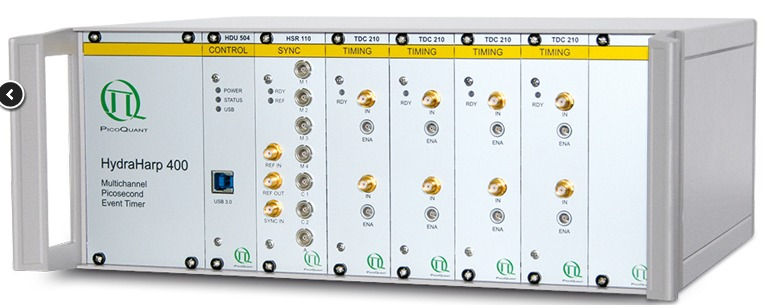
\includegraphics[width=.5\linewidth]{hydraharp}
  \centering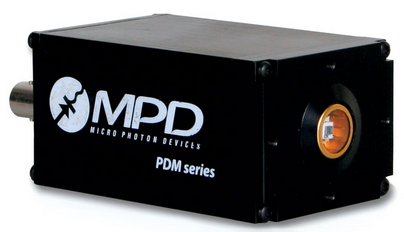
\includegraphics[width=.5\linewidth]{spad}
  \caption{HydraHarp et détecteur SPAD}
  \label{fig:hydraharp}
\end{figure}

\subsection{Logiciel du constructeur}

\subsection{Matlab}

\begin{lstlisting}[frame=single,caption={Exemple d'utilisation de HydraHarp avec Matlab},label={lst:exhydraharp},breaklines=true,]  % Start your code-block

???
\end{lstlisting}

%----------------------------------------------------------------------------------------

\section{Lockin Zurich Instruments}\index{Lockin Zurich Instruments}

\subsection{Matlab}

\begin{lstlisting}[frame=single,caption={Exemple d'utilisation du lockin Surich Instruments avec Matlab},label={lst:exlockinzi},breaklines=true,]  % Start your code-block
  
???
\end{lstlisting}

%----------------------------------------------------------------------------------------

\section{Matisse}\index{Matisse}

Le Matisse (figure~\ref{fig:matisse}) donne un laser de longueur d'onde ajustable dans une plage d'environ 100 nm.
La puissance de sortie est de l'ordre de 2 watts.

On peut contrôler le Matisse avec le logiciel du constructeur où avec Python.
Les deux manières étant mutuellement exclusives\footnote{Les deux peuvent sembler fonctionner ensemble pendant un long moment, mais on aura d'éventuelles erreurs dans le code Python.}.

\begin{figure}[h]
  \centering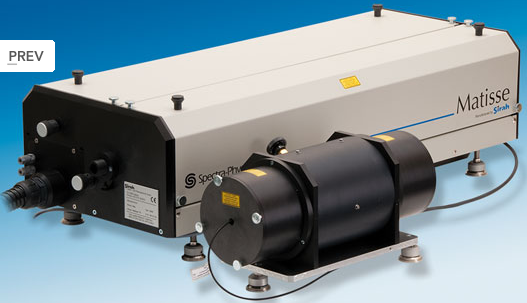
\includegraphics[width=.5\linewidth]{matisse}
  \caption{Matisse et cellule de référence}
  \label{fig:matisse}
\end{figure}

\subsection{Logiciel du contructeur}

Étant donné des choix de conception de Sirah, chaque Matisse doit être contrôlé avec son propre logiciel.
On ne peut pas interchanger les deux lasers parce que le logiciel stoque la configuration de son laser attitré.
Pour une raison apparentée, on ne peut pas contrôler les deux lasers avec le même ordinateur\footnote{Le code Python permet de contrôler les deux lasers en même temps.}.

\subsection{Python}

La classe Matisse sert à interagir avec le laser Matisse.
On peut contrôler les deux Matisses (éventuellement en même temps) avec Python.
%Il s'agit d'une classe très ciblée puisqu'en dehors de l'initialisation on ne peut faire qu'une chose: mesurer.
Voir Code~\ref{lst:exmatisse} pour un exemple d'utilisation.

\begin{lstlisting}[frame=single,caption={Exemple d'utilisation du Matisse avec Python},label={lst:exmatisse},breaklines=true,]  % Start your code-block

# importe le module
import Matisse

\end{lstlisting}

%----------------------------------------------------------------------------------------

\section{Millenia}\index{Millenia}

Le Millenia (figure~\ref{fig:millenia}) sert à pomper le Matisse.

La facon la plus simple d'utiliser ce laser est en mode manuel où les parametres sont ajustés au moyen de la boite de contrôle.
On peut également contrôler 

\begin{figure}[h]
\centering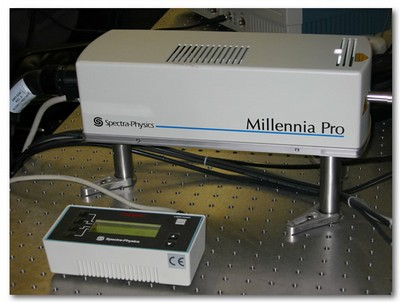
\includegraphics[width=.5\linewidth]{milleniaPro}
\caption{Millenia}
\label{fig:millenia}
\end{figure}

%----------------------------------------------------------------------------------------

\section{Racal Dana}\index{Racal Dana}

L'appareil Racal Dana 1991 (figure \ref{fig:racaldana}) est utilisé comme compteur de photon.
Sa configuration manuelle est difficile; c'est pourquoi on préfère le configurer de facon logicielle.
On établi donc la communication avec l'appareil à partir d'un ordinateur et on lui envoie les commandes appropriées.

Pour pouvoir bien fonctionner, le compteur de photon a besoin d'une référence temporelle.
Pour ce faire, nous utilisons la sortie ??? comme entrée de {\it Input B} ???.
Le comptage se fait proprement dit sur l'entrée {\it Input 1} ???.

Cet appareil possède deux interfaces logicielles soient Matlab et Python.

\begin{figure}[h]
\centering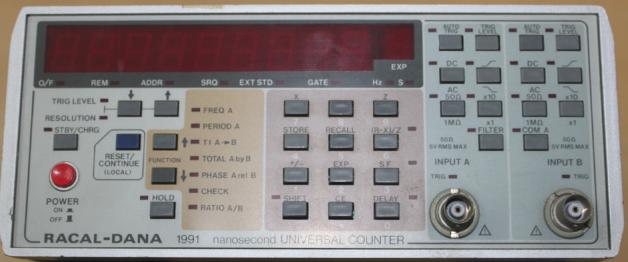
\includegraphics[width=.5\linewidth]{RacalDana1991}
\caption{Racal Dana 1991}
\label{fig:racaldana}
\end{figure}

\subsection{Matlab}

\subsection{Python}

La classe RacalDana sert à interagir avec le compteur de photon Racal Dana 1991.
Il s'agit d'une classe très ciblée puisqu'en dehors de l'initialisation on ne peut faire qu'une chose: mesurer.
Voir Code~\ref{lst:exracaldana} pour un exemple d'utilisation.

\begin{lstlisting}[frame=single,caption={Exemple d'utilisation de {\it RacalDana avec Python}},label={lst:exracaldana},breaklines=true,]  % Start your code-block
 
import racalDana  # importe le module

# initialise la communication (on suppose l'adresse GPIB 3)
compteur = racalDana.RacalDana('GPIB0::3::INSTR') 

# mesure pendant 5 secondes
comptes = compteur.measure(exposureTime=5)
\end{lstlisting}

%----------------------------------------------------------------------------------------

\section{SP275}\index{SP275}

\subsection{Matlab}

\begin{lstlisting}[frame=single,caption={Exemple d'utilisation du SP275 avec Matlab},label={lst:exsp275},breaklines=true,]  % Start your code-block

???
\end{lstlisting}

\subsubsection{Détecteurs}

%----------------------------------------------------------------------------------------

\section{SR400}\index{SR400}

\subsection{Matlab}

\begin{lstlisting}[frame=single,caption={Exemple d'utilisation du SR400 avec Matlab},label={lst:exsr400},breaklines=true,]  % Start your code-block

???
\end{lstlisting}

%----------------------------------------------------------------------------------------

\section{SR830}\index{SR830}

%----------------------------------------------------------------------------------------

\section{Trivista}\index{Trivista}

\subsection{Matlab}

\begin{lstlisting}[frame=single,caption={Exemple d'utilisation du Trivista avec Matlab},label={lst:extrivista},breaklines=true,]  % Start your code-block

???
\end{lstlisting}

%----------------------------------------------------------------------------------------

\section{Verdi}\index{Verdi}

%----------------------------------------------------------------------------------------

\section{Wavemeter}\index{Wavemeter}

Le Wavemeter sert à donner une mesure précise de la longueur d'onde du laser sortant du Matisse.

\subsection{Lecture}
Il est possible de lire la longueur d'onde mesurée par l'instrument en utilisant deux faux ports série.
Sur windows, il faut installer le logiciel {\it com0com}\footnote{\url{http://com0com.sourceforge.net}}.
On crée ensuite deux ports séries (com 90 et com 91) reliés ensemble.
Le logiciel du Wavemeter écrit ses résultats sur com 90 (???).
Ce dernier recopie tout sur com 91.
Il suffit de lire les résultats sur com 91.
Un exemple de code est donné dans Code~\ref{lst:exwavemeter}.

Cette fonction est implémentée dans la classe Matisse, dans la fonction (en fait une propriété) realWavelength.

\subsection{Python}

\begin{lstlisting}[frame=single,caption={Exemple d'utilisation du Wavemeter avec Python},label={lst:exwavemeter},breaklines=true,]  % Start your code-block

import Matisse
laser = Matisse.Matisse()

print(laser.realWavelength)
\end{lstlisting}


%----------------------------------------------------------------------------------------
%	CHAPTER 3
%----------------------------------------------------------------------------------------

\chapterimage{laser} % Chapter heading image

\chapter{Expériences}

\section{Absorption (UV)}\index{Absorption (UV)}

%----------------------------------------------------------------------------------------
\section{micro-Photoréflectance}\index{micro-Photoréflectance}

%----------------------------------------------------------------------------------------
\section{micro-Raman}\index{micro-Raman}

%----------------------------------------------------------------------------------------
\section{Photoluminescence}

%----------------------------------------------------------------------------------------
\subsection{Trivista}\index{Photoluminescence (Trivista)}

%----------------------------------------------------------------------------------------
\subsection{U1000}\index{Photoluminescence (U1000)}

%----------------------------------------------------------------------------------------
\section{Photoluminescence résolue temporellement}\index{Photoluminescence résolue temporellement}

%----------------------------------------------------------------------------------------
\section{Raman}\index{Raman}



%----------------------------------------------------------------------------------------
%	INDEX
%----------------------------------------------------------------------------------------

\cleardoublepage
\phantomsection
\setlength{\columnsep}{0.75cm}
\addcontentsline{toc}{chapter}{\textcolor{ocre}{Index}}
\printindex

%----------------------------------------------------------------------------------------

\end{document}
